\documentclass[10pt,final,journal,a4paper,twoside,twocolomn]{IEEEtran}
\usepackage{stmaryrd}
\usepackage[cmex10]{amsmath}
\interdisplaylinepenalty=2500
\usepackage{graphicx}
%%%%%%%%%%%%%%%%%%%%%%%%%%%%%%%%%%%%%%%%%%%%%%%%%%%%%%%%%%%%%%%%%%%%%%%%
\begin{document}
\title{Argon Plasma-Induced Quantum Well Intermixing for
       Monolithic Photonic Integration}
\author{Xin~Zhang
        and~Jian-Jun~He,~\IEEEmembership{Senior~Member,~IEEE}
\thanks{Manuscript received September 1, 2009; revised September 9, 2009.}
\thanks{X.~Zhang is with
        the Center for Optical and Electromagnetic Research,
        State Key Laboratory of Modern Optical Instrumentation,
        Zhejiang University, Hangzhou 310058, China.}
\thanks{J.-J.~He is with
        the Center for Optical and Electromagnetic Research,
        State Key Laboratory of Modern Optical Instrumentation,
        Zhejiang University, Hangzhou 310058, China.
        He is also with Lightip Technologies, Inc., Ottawa,
        ON K1K 4R8, Canada (e-mail: jj.he@lightip.com).}
\thanks{Digital Object Identifer 00.0001/LPT.2010.000001}}
\markboth{IOE PHOTONICS TECHNOLOGY LETTERS, VOL.~1,NO.~1,September~9,~2010}
         {X.~Zhang \MakeLowercase{\textit{et al.}}:
         Argon Plasma-Induced Quantum Well Intermixing for Monolithic Photonic Integration}
\IEEEspecialpapernotice{(Year I Paper)} \maketitle
%%%%%%%%%%%%%%%%%%%%%%%%%%%%%%%%%%%%%%%%%%%%%%%%%%%%%%%%%%%%%%%%%%%%%%%%
\begin{abstract}
Models and formulations needed for the calculation of the optical
properties of the diffused quantum wells are analyzed in this paper.
\end{abstract}
\begin{IEEEkeywords}
Photonic integrated circuits (PICs), quantum well intermixing (QWI),
polarization independence.
\end{IEEEkeywords}
%%%%%%%%%%%%%%%%%%%%%%%%%%%%%%%%%%%%%%%%%%%%%%%%%%%%%%%%%%%%%%%%%%%%%%%%
\section{Introduction}
\chapter{����}

\section{��ͨ������Ӽ��ɻ�·}

\section{�����ĵ���Ҫ�о�����}

\section{Theoretical Analysis}
\subsection{Diffusion Model}
Interdiffusion of atoms across the heterointerface alters the
composition profile across the QW structure. Mathematical models are
needed to describe and calculate the changes in the composition
profile as a function of the duration of interdiffusion. In the
section, we adopt the notation $A_{x}B_{1-x}C_{y}D_{1-y}$ to denote
the chemical formula of a III-V semiconductor material, where A and
B represent the Group III atoms, and C and D represent the Group V
atoms respectively. After interdiffusion the mole fractions of Group
III and V atoms are function of position along the direction of
crystal growth (the $z$-direction) and are denoted by $w(z)$ and
$v(z)$.

The diffusion process is usually described by the Fick's Second Law
in the direction of crystal growth
\begin{equation}
\frac{\partial{C}}{\partial{t}}=D\frac{\partial^2{C}}{\partial{z^2}}
\end{equation}
where $C$ denotes the concentration of the atoms and $D$ is the
diffusion coefficient. The diffusion coefficient of the atoms is
usually assumed to be identical in the quantum well. The
interdiffusion process is characterized by a diffusion length $L_d$,
which is defined as $L_d=\sqrt{Dt}$, where $D$ is the diffusion
coefficient and $t$ is the annealing time of the thermal processing.
Consider a single
$In_{wx}Ga_{1-wx}As_{wy}P_{1-wy}/In_{bx}Ga_{1-bx}As_{by}P_{1-by}$
quantum well, the composition profile of In and As in this QW after
interdiffusion are given by
\begin{eqnarray}
    w(z)&=&wx-\frac{bx-wx}{2} \notag\\
        &&\times \biggr[2-\textrm{erf}\biggr(\frac{L_z+2z}{4L_d^{III}}\biggr)
        -\textrm{erf}\biggr(\frac{L_z-2z}{4L_d^{III}}\biggr)\biggr]
\end{eqnarray}

\begin{eqnarray}
    v(z)&=&wy-\frac{by-wy}{2} \notag\\
        &&\times \biggr[2-\textrm{erf}\biggr(\frac{L_z+2z}{4L_d^{V}}\biggr)
        -\textrm{erf}\biggr(\frac{L_z-2z}{4L_d^{V}}\biggr)\biggr]
\end{eqnarray}

In this case, interdiffusion can occur on both group III and V
sublattices, which are characterized by their diffusion lengths
$L_d^{III}$ and $L_d^V$, respectively. The diffusion length ratio,
i.e., $k=L_d^V/L_d^{III}$, depends on the details of interdiffusion
process and is still an open question which requires further
studies.

\subsection{Band Structure}
The optical properties of a non-square interdiffused quantum well
depend on the band structure which can be found by using some
existing models, such as the envelop function approximation,
pseudopotential method, the tight-binding model and the effective
bond-orbital model. We use the envelop function approximation
because of the computationally simplicity and enough accuracy for
describing phenomena occurring on a length scale large compared with
the unit cell of the crystal. The envelop function for the
z-direction can be obtained by solving the Schrodinger-like equation
shown below.
\begin{equation}\label{schrodinger}
    \frac{-h^2}{2} \frac{d}{dz} \frac{1}{m_\perp^*(z)} \frac{d\varphi(z)}{dz}
    +V(z)\varphi(z)
        = E\varphi(z)
\end{equation}
where $m_\perp(z)$ is the effective mass of the
conduction band or valence band. $V(z)$ is the position-dependent
potential energy of the conduction band heavy hole valence band
or light hole valence band, which can be determined by Equation
\ref{V_c}-\ref{V_LH}, respectively.
This differential equation is solved using the
finite-difference method (FDM) with appropriate boundary conditions.
Usually we consider the quantum well contained in a large box along
the z-direction with the boundary condition $\varphi=0$ at the
boundaries of the box.
\begin{equation}\label{V_c}
    V_c(z)
        = Q_c Eg(z) - (1-Q_c)S_\perp(z)
\end{equation}

\begin{equation}\label{V_HH}
    V_{HH}(z)
        = (1-Q_c)[Eg(z) - S_\perp(z)] + S_\parallel(z)
\end{equation}

\begin{eqnarray}\label{V_LH}
    V_{LH}(z)&=& (1-Q_c)[Eg(z) - S_\perp(z)] \notag\\
    && +0.5[S_\parallel(z) + \Delta_0(z)] \notag\\
    && -0.5 \sqrt{9S_\parallel^2(z)-2S_\parallel^2(z)\Delta_0(z)+\Delta_0^2(z)}
\end{eqnarray}

The calculation of the potential energy has take consideration
the strain effect of the quantum well materials by
Equation \ref{S_perp}-\ref{epsilon}.
All the material parameters for the numerical calculation can be obtained
from Table \ref{parametertable} by \cite{table}.
\begin{equation}\label{S_perp}
    S_\perp(z)
        = -2a_v(z)[1-\frac{C_{12}(z)}{C_{11}(z)}] \epsilon(z)
\end{equation}
\begin{equation}\label{S_parallel}
    S_\parallel(z)
        = -b(z)[1+\frac{2C_{12}(z)}{C_{11}(z)}] \epsilon(z)
\end{equation}
\begin{equation}\label{a_v}
    a_v(z)
        = -\frac{1}{3}[C_{11}(z)+2C_{12}(z)] \frac{dEg}{dp}(z)
\end{equation}
\begin{equation}\label{epsilon}
    \epsilon(z)
        = \frac{a_{InP}(z)-a(z)}{a(z)}
\end{equation}

\begin{table*}[!t]
    \renewcommand{\arraystretch}{1.3}
    \caption{Material parameters for InGaAsP used in numerical calculation
        at room temperature (300K) of Quantum Wells structures}
    \centering
    \label{parametertable}
    \begin{tabular}{llll}
        \hline
        \hline
        Symbol & Parameter & $In_{x}Ga_{1-x}As_{y}P_{1-y}$ & Unit\\
        \hline
        $Q_c:Q_v$ & Band offset splitting ratio & $0.6:0.4$ & $-$\\
        $E_g(z)$ & Energy bandgap & $1.35-1.17y+0.668(1-x)-0.069y(1-x)+0.18y^2$ & eV\\
                                  && $+0.03(1-x)y^2+0.758(1-x)^2-0.322y(1-x)^2$ &\\
        $\Delta_0(z)$ & Spin-orbit splitting & $0.34(1-x)y+0.43xy+0.10(1-x)(1-y)+0.10x(1-y)$ & eV\\
        $m_e$ & Electron mass & $0.91095\times10{-30}$ & kg\\
        $m_c^*(z)$ & Electron effective mass & $0.0632(1-x)y+0.0213xy+0.17(1-x)(1-y)+0.077x(1-y)$ & $m_e$\\
        $m_{\perp HH}^*(z)$ & Heavy hole effective mass & $0.5(1-x)y+0.41xy+0.54(1-x)(1-y)+0.12x(1-y)$ & $m_e$\\
                            & perpendicular to QW layer &&\\
        $m_{\perp LH}^*(z)$ & Light hole effective mass & $0.088(1-x)y+0.024xy+0.16(1-x)(1-y)+0.12x(1-y)$ & $m_e$\\
                            & perpendicular to QW layer &&\\
        $m_{\parallel HH}^*(z)$ & Heavy hole effective mass & $0.11(1-x)y+0.031xy+0.19(1-x)(1-y)+0.15x(1-y)$ & $m_e$\\
                                & parallel to QW layer &&\\
        $m_{\parallel LH}^*(z)$ & Light hole effective mass & $0.23(1-x)y+0.082xy+0.34(1-x)(1-y)+0.29x(1-y)$ & $m_e$\\
                                & parallel to QW layer &&\\
        $a(z)$ & Lattice constant & $0.56533(1-x)y+0.60584xy+0.54512(1-x)(1-y)+0.58688x(1-y)$ & nm\\
        $C_{11}(z)$ & Elastic stiffness constant & $11.8(1-x)y+8.329xy+14.12(1-x)(1-y)+10.22x(1-y)$ & $10^{11}dyn/cm^2$\\
        $C_{12}(z)$ & Elastic stiffness constant & $5.38(1-x)y+4.526xy+6.253(1-x)(1-y)+5.76x(1-y)$ & $10^{11}dyn/cm^2$\\
        $dE_g/dP(z)$ & Hydrostatic pressure coefficient & $11.5(1-x)y+10.0xy+11.0(1-x)(1-y)+8.5x(1-y)$ & $10^{-6}eV/bar$\\
        $b(z)$ & Shear deformation potential & $-1.7(1-x)y-1.8xy-1.5(1-x)(1-y)-2.0x(1-y)$ & eV\\
        \hline
        \hline
    \end{tabular}
\end{table*}

To show the validity of the theoretical model, I adopt the data by Nanyang
Technology University with the same method of argon plasma-induced QWI \cite{redshift}.
The layer structure of samples used in the experiment is shown in Table \ref{RedShiftSample}.
Figure \ref{ex_redshift} shows the PL spectra of one InP cap sample before plasma exposure
and after plasma exposure followed by several rapid thermal annealing (RTA) process.
The result shows that after argon plasma exposure, both the blueshift and redshift
of the bandgap can be obtained by controlling the temperature of RTA.

\begin{table}[!t]
    \renewcommand{\arraystretch}{1.3}
    \caption{The layer structure for the undoped InGaAsP/InP single quantum well}
    \centering
    \label{RedShiftSample}
    \begin{tabular}{cccc}
        \hline
        \hline
        No. & Composition & Thickness(nm) & Layer\\
        \hline
        5 & $In_{0.53}Ga_{0.47}As$ & 500 & Buffer/cap\\
        4 & InP & 500 & Barrier/cap\\
        3 & $In_{0.71}Ga_{0.29}As_{0.61}P_{0.39}$ & 3.5 & Well\\
        2 & InP & 300 & Barrier\\
        1 & InP & $-$ & substrate\\
        \hline
        \hline
    \end{tabular}
\end{table}

\begin{figure}[!t]
    \centering
    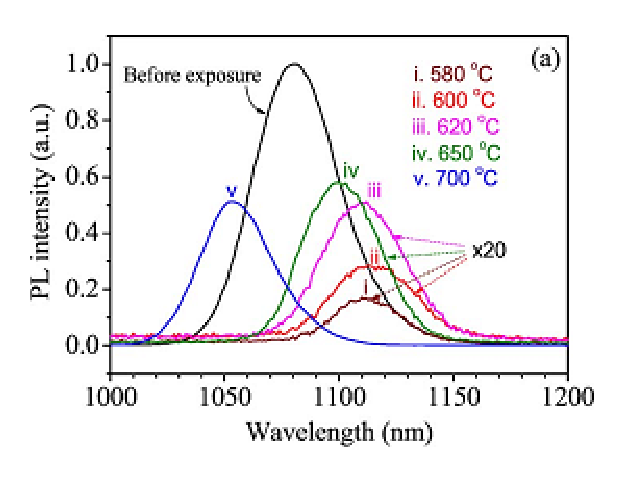
\includegraphics[width=2.5in]{fig/exp_red}
    \caption{PL spectra for one InP cap sample before plasma exposure and after plasma
        exposure followed by annealing at (i) 580$^\circ$C, (ii) 600$^\circ$C, (iii) 620$^\circ$C,
        (iv) 650$^\circ$C, (v) 700$^\circ$C.}
    \label{ex_redshift}
\end{figure}

To interpret the above observations of bandgap modification,
the wavelength shift of the interdiffused QW structure was calculated using
my theoretical model. Figure \ref{my_redshift} shows the calculated PL peak
wavelength shift as a function of group III diffusion length under different k
parameters. It can be seen that, in this QW structure, an observable redshift
can be obtained only when k$<$0.63 roughly; i.e., the group III sublattice must
interdiffuse about twice as fast as the group V sublattice.

\begin{figure}[!t]
    \centering
    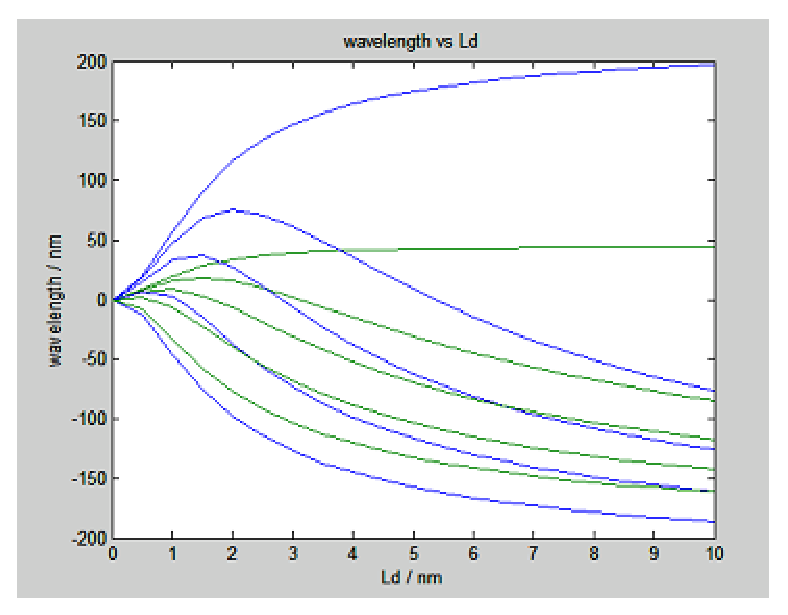
\includegraphics[width=2.5in]{fig/red}
    \caption{The calculated wavelength shift of the ground state transition
        as a function of the group III diffusion length under different k parameters.}
    \label{my_redshift}
\end{figure}

\subsection{Optical Absorption}
Subsection text here.

\subsection{Quantum Confined Stark Effects}
Subsection text here.
\begin{equation}\label{QCSE}
    \frac{-h^2}{2}
    \frac{d}{dz}
    \frac{1}{m_\perp^*(z)}
    \frac{d\varphi(z)}{dz}
    +[V(z)+zeE]\varphi(z)
        = E\varphi(z)
\end{equation}

\subsection{Optical Gain}
Subsection text here.
\begin{eqnarray}
    g(\hbar\omega) &=& \frac{2 m_r \omega}{n_{eff} c \varepsilon_0 \pi \hbar^2 L_z}
        \sum_{n,m} \int_0^\infty dE_\parallel |e\cdot M_{cv}(E_\parallel)|^2 \notag\\
    && \times \frac{\frac{\hbar}{\pi \tau_{in}}}
        {(E_{en}-E_{hm}+E_\parallel-\hbar\omega)^2+(\frac{\hbar}{\pi \tau_{in}})^2} \notag\\
    && \times [f_c^n(E_\parallel)-f_v^m(E_\parallel)]
\end{eqnarray}

\subsection{Refractive Index}
Subsection text here.
\begin{eqnarray}
    \Delta n(\hbar\omega) &=& \frac{m_r}{n_{eff} c \varepsilon_0 \pi \hbar^2 L_z}
        \sum_{n,m} \int_0^\infty dE_\parallel |e\cdot M_{cv}(E_\parallel)|^2 \notag\\
    && \times \frac{E_{en}-E_{hm}+E_\parallel-\hbar\omega}
        {(E_{en}-E_{hm}+E_\parallel-\hbar\omega)^2+(\frac{\hbar}{\pi \tau_{in}})^2} \notag\\
    && \times [f_c^n(E_\parallel)-f_v^m(E_\parallel)]
\end{eqnarray}


\section{Experiments}
\subsection{Parameters Affecting the Bandgap Energy Shifts in QWI}
Parameters affecting the bandgap energy shifts in argon
plasma-induced quantum well intermixing have previously been studied
in detail elsewhere \cite{icpparam}. Inductively coupled plasma
(ICP) parameters, RTA parameters and QW layer structure are three
main factors affects the magnitude of bandgap energy shifts. In my
experiments, ICP and RTA parameters were investigated.

\begin{table}[!t]
    \renewcommand{\arraystretch}{1.3}
    \caption{The layer structure for the 0.9\% compressive strain
        InGaAsP/InGaAsP multiple quantum well}
    \centering
    \label{mySample}
    \begin{tabular}{cccc}
        \hline
        \hline
        Layer & Composition & Thickness(nm) & Doping(cm$^{-3}$)\\
        \hline
        Sacrificial & InP                          & 500  & Zn\\
        Cap         & p$^+$-InGaAs                 & 200  & Zn:1e19\\
        Cladding    & p-InP                        & 1500 & Zn:1e18\\
        Etch-stop   & p-InGaAsP (1.24um)           & 10   & Zn:4e17\\
        Cladding    & p-InP                        & 150  & Zn:4e17\\
        GRINSCH     & p-InGaAsP (1.05um)           & 20   & Zn:4e17\\
        GRINSCH     & p-InGaAsP (1.15um)           & 20   & Zn:4e17\\
        GRINSCH     & p-InGaAsP (1.24um)           & 20   & Zn:4e17\\
        QW                 & InGaAsP               & 5    & $-$\\
        Barrier$\times$7   & InGaAsP (1.24um)      & 10   & $-$\\
        QW$\times$7        & InGaAsP               & 5    & $-$\\
        GRINSCH     & p-InGaAsP (1.24um)           & 20   & Si:4e17\\
        GRINSCH     & p-InGaAsP (1.15um)           & 20   & Si:4e17\\
        GRINSCH     & p-InGaAsP (1.05um)           & 20   & Si:4e17\\
        Buffer      & n-InP                        & 1500 & Si:2e18\\
        Substrate   & n$^+$-InP                    & $-$  & S or Sn:~4e18\\
        \hline
        \hline
    \end{tabular}
\end{table}
The layer structure of the QW samples is shown in Table
\ref{mySample}. The plasma source generator used in the experiments
was a Plasmalab System 100, which was built by Oxford Instruments.
The ICP parameters were optimized using 80-sccm Ar flow rate,
80-mtorr chamber pressure, 480-w RF power, 500-w ICP power,
20$^\circ$C temperature, 1-min time. After Ar plasma exposure, the
samples were annealed at 600$^\circ$C-800$^\circ$C for 2 min in a
rapid thermal processer (RTP) in a nitrogen atmosphere. Two fresh
pieces of InP were used to provide an phosphorous over-pressure
environment during the annealing process and further to prevent the
sample surface from phosphorous outdiffusion. Room-temperature (RT)
Photoluminescence (PL) measurements were then performed to obtain
the bandgap energy shifts data.

\begin{figure}[!t]
    \centering
    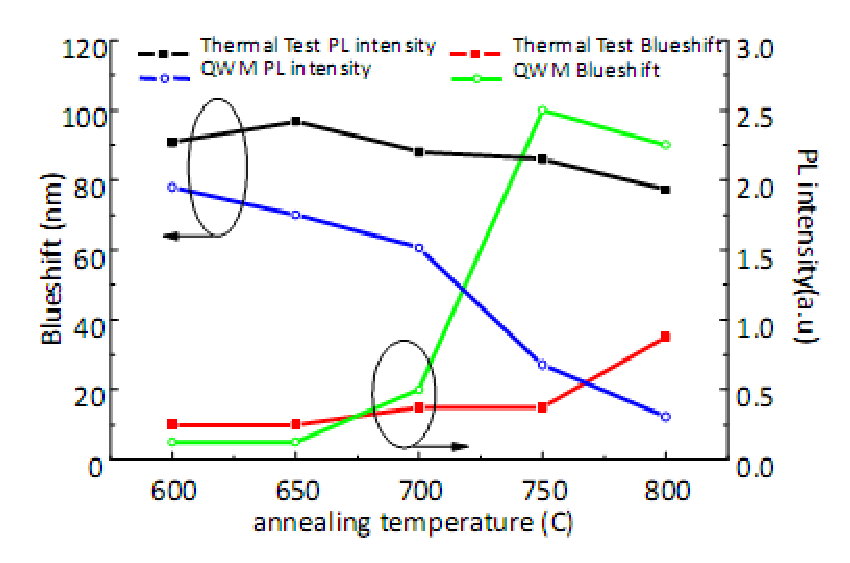
\includegraphics[width=2.5in]{fig/rta1}
    \caption{Bandgap blue shift and PL peak intensity vs. RTA temperature}
    \label{ex_rta1}
\end{figure}
Figure \ref{ex_rta1} shows the bandgap blue shift and PL peak
intensity in different RTA temperature. Large bandgap shift of
\~90nm is obtained under RTA temperature of 750$^\circ$C, while the
PL peak intensity decrease of 80\% is slight and acceptable.

\begin{figure}[!t]
    \centering
    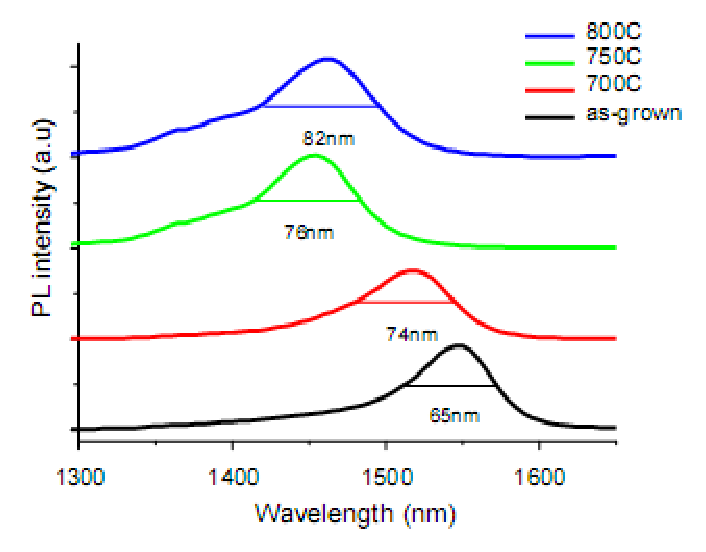
\includegraphics[width=2.5in]{fig/rta2}
    \caption{PL vs. wavelength}
    \label{ex_rta2}
\end{figure}
Figure \ref{ex_rta2} shows the full width at half maximum (FWHM) of
the PL under different RTA temperature. The slight linewidth
broadening may result from different bandgap blue shift of TE and TM
modes of the PL.

\subsection{Waveguiding Characteristics}
Subsection goes here.

In order to investigate the effect of argon plasma on waveguide quality,
waveguide loss measurement using the Fabry-Perot fringe technique were
performed. 3-$\mu$m-wide ridge waveguides were fabricated on the intermixed
region. The sample was then cleaved to form a 1-mm-long Fabry-Perot cavity.
A tunable (1.45-1.59$\mu$m) laser diode was used for the absorption experiments.
The light was modulated at 10KHz and coupled into the TE mode of the
waveguide through a tapered polarization preserving fiber. The transmitted
light was then captured by a similar fiber coupled to a Ge-detector followed
by a lock-in amplifier.

\begin{figure}[!t]
    \centering
    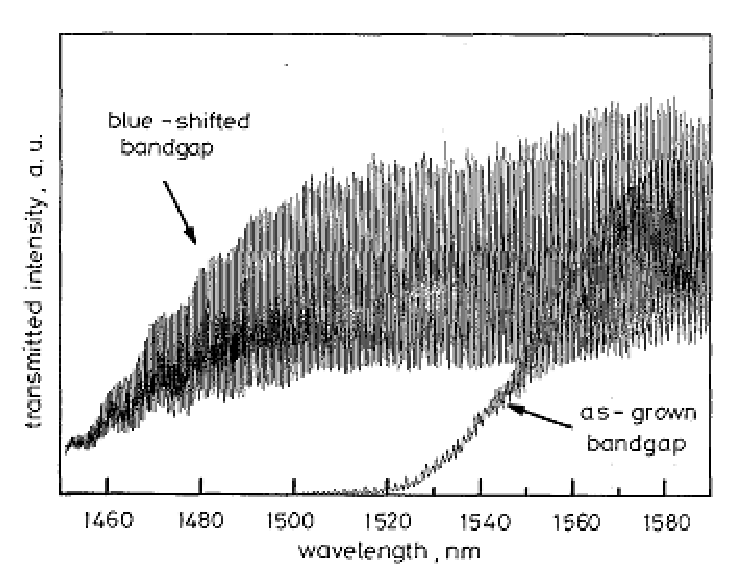
\includegraphics[width=2.5in]{fig/waveguide1}
    \caption{Measured transmission spectra of blue-shifted waveguide}
    \label{ex_waveguide1}
\end{figure}
Figure \ref{ex_waveguide1} shows the measured transmitted spectra of the blue-shift
waveguide cavity. Fabry-Perot interference fringes were formed due to multiple
reflections at the cleaved facets. From the contrast of these fringe the waveguide
loss can be determined by Equation \ref{loss},

\begin{equation}\label{loss}
    L=10\lg\Big[\frac{1}{\sqrt{R_1R_2}}\frac{1}{K_m}(1-\sqrt{1-K_m^2})\Big]
\end{equation}
where $R_1$ and $R_2$ are the reflectivity of the cleaved facets
and $K_m$ is the contrast of the fringes.

\begin{figure}[!t]
    \centering
    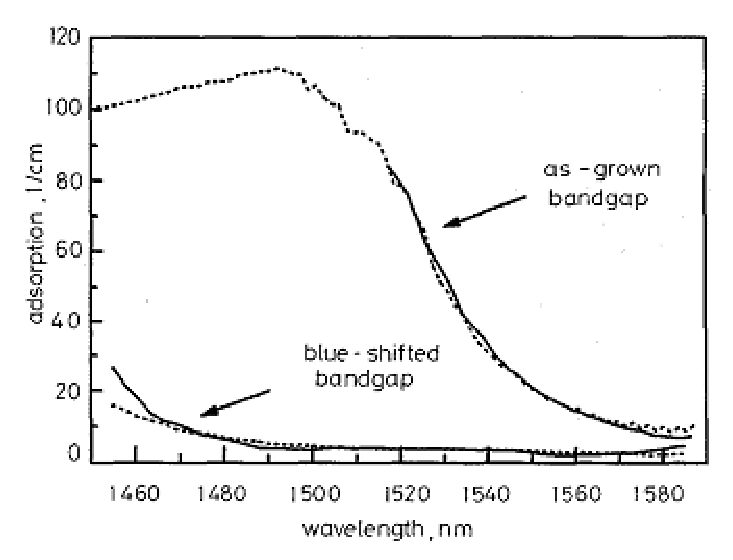
\includegraphics[width=2.5in]{fig/waveguide2}
    \caption{Absorption constants derived from measured transmission spectra
        using modulation ratio and average transmission intensity for
        blue-shifted waveguide}
    \label{ex_waveguide2}
\end{figure}
Figure \ref{ex_waveguide2} presents the absorption as a function of wavelength
derived from Figure \ref{ex_waveguide1} and Equation \ref{loss}.

\subsection{Electrical Characteristics}
\begin{figure}[!t]
    \centering
    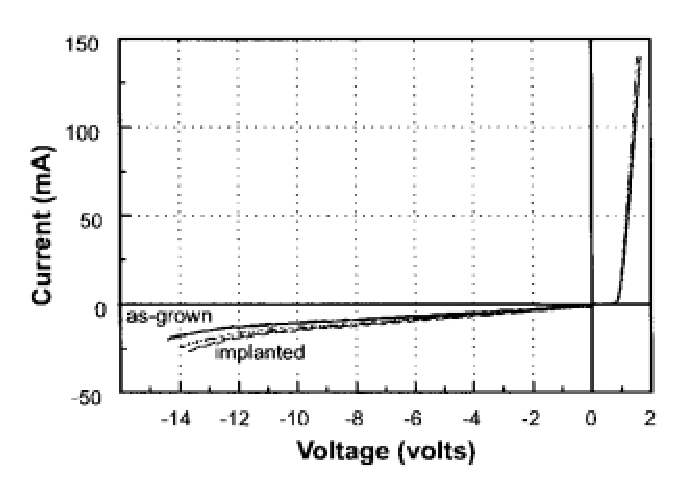
\includegraphics[width=2.5in]{fig/iv}
    \caption{I-V characteristics of p-i-n diodes made from as-grown and blue-shift materials}
    \label{ex_iv}
\end{figure}
For the Ar plasma-induced QWI process to be a useful technique for
lateral bandgap control in monolithic integration, it is essential
that the electrical characteristics of the p-i-n structure not be
degraded by the Ar plasma and/or anneal. Figure llll shows the
current versus voltage (I-V) characteristics for the as-grown and
blue-shift materials following a 120-s RTA at 750 $^\circ$C. We see
that all samples have very similar I-V characteristics.

\subsection{Carrier Induced Tuning Characteristics}
tuning? is vital!


\section{Application of QWI}
\subsection{Bandgap tuning of InP-Based Lasers}
\subsection{Extended Cavity Laser}

\section{Conclusion}
The conclusion\cite{tex} goes here\cite{zz}.

%%%%%%%%%%%%%%%%%%%%%%%%%%%%%%%%%%%%%%%%%%%%%%%%%%%%%%%%%%%%%%%%%%%%%%%%
\begin{thebibliography}{99}
\bibitem{JMarsh}
John~H.~Marsh,
\newblock "Quantum well Intermixing"
\newblock {\em Semlcond. Sci. Technol}, vol.8, pp.1136-1155, 1993.

\bibitem{IIID}
Sylvain Charbonneau, Emil S. Koteles, P. J. Poole, J. J. He, G. C.
Aers, J. Haysom, M. Buchanan, Y. Feng, A. Delage, F. Yang, M.
Davies, R. D. Goldberg, P. G. Piva, and I. V. Mitchell,
\newblock "Photonic Integrated Circuits Fabricated Using Ion Implantation"
\newblock {\em IEEE JOURNAL OF SELECTED TOPICS IN QUANTUM ELECTRONICS}, vol.4, no.4, pp.772-793, 1998.

\bibitem{IFVD}
B. S. Ooi, K. McIlvaney, M. W. Street, A. S. Helmy, S. G. Ayling, A.
C. Bryce, J. H. Marsh, and J. S. Roberts,
\newblock "Selective quantum-well intermixing in GaAs�CAlGaAs structures using impurity-free vacancy diffusion"
\newblock {\em IEEE J. Quantum Electron}, vol. 33, no. 10, pp. 1784�C1793, Oct. 1997.

\bibitem{SiO2}
S. P. McDougall, O. P. Kowalski, C. J. Hamilton, F. Camacho, B. Qiu,
M. Kee, R. M. De La Rue, A. C. Bryce, and J. H. Marsh,
\newblock "Monolithic integration via a universal damage enhanced quantum well intermixing technique"
\newblock {\em IEEE J. Sel. Topics Quantum Electron}, vol. 4, no. 4, pp. 636�C646, Jul./Aug. 1998.

\bibitem{PAID}
B. S.Ooi, T.K.Ong, andO.Gunawan,
\newblock "Multiple-wavelength integration in InGaAs�CInGaAsP structures using pulsed laser irradiation
induced quantum well intermixing"
\newblock {\em IEEE J. Quantum Electron.}, vol. 40, no. 5, pp. 481�C490, May 2004.

\bibitem{ArPlasma}
H. S. Djie, T. Mei, J. Arokiaraj, C. Sookdhis, S. F. Yu, L. K. Ang,
and X. H. Tang,
\newblock "Experimental and Theoretical Analysis of Argon Plasma-Enhanced Quantum-Well Intermixing"
\newblock {\em IEEE JOURNAL OF QUANTUM ELECTRONICS}, VOL. 40, NO. 2, pp.166-174, Feb. 2004

\bibitem{40G}
James~W.~Raring and Larry~A.~Coldren,
\newblock "40-Gb/s Widely Tunable Transceivers"
\newblock {\em IEEE JOURNAL OF SELECTED TOPICS IN QUANTUM ELECTRONICS}, vol.13, no.1, pp.3-14, 2007.

\bibitem{table}
\newblock {\em IEE Proc.-Optoelectron}, vol.149, no.4, August, 2002.

\bibitem{redshift}
D.~Nie, T.~Mei, X.~H.~Tang {\em et al}
\newblock "Argon plasma exposure enhanced intermixing in an undoped InGaAsP/InP quantum-well structure"
\newblock {\em J. Applied Physics}, 100, 046103, 2006

\bibitem{icpparam}
D.~Leong, H.~S.~Djie and P.~Dowd,
\newblock "A New Quantum Well Intermixing Technique Using Inductively Coupled
    Argon Plas ma on InGaAs/InGaAsP laser structures"

\bibitem{tex}
H.~Kopka and P.~W. Daly, \emph{A Guide to \LaTeX}, 3rd~ed.\hskip 1em
plus 0.5em minus 0.4em\relax Harlow, England: Addison-Wesley, 1999.

\bibitem{zz}
Banerjee M, Pal S.~K.
\newblock Roughness of fuzzy set.
\newblock {\em Information Sciences}, 93:235$\sim$246, 1996.

\end{thebibliography}
%%%%%%%%%%%%%%%%%%%%%%%%%%%%%%%%%%%%%%%%%%%%%%%%%%%%%%%%%%%%%%%%%%%%%%%%
\begin{IEEEbiographynophoto}{Xin~Zhang}
was born in Zhejiang Province, China, in April 1986. He received the
B.Eng. degree in information engineering from Zhejiang University,
Zhejiang, China, in 2009. He is currently working toward the PhD
degree in optical engineering at the same university. His current
research interests are in the areas of design, optimization, and
fabrication of photonic integrated circuits for optical
communications systems.

\end{IEEEbiographynophoto}

\begin{IEEEbiographynophoto}{Jian-Jun~He}
received both the Diplome d��Etudes Approfondies and Ph.D. degrees
in semiconductor optoelectronics from the University of Paris VI,
Paris, France, in 1986 and 1989, respectively. From 1986 to 1989, he
worked at Center National d��Etudes des T��l��communications,
Bagneux, France, on acoustooptical devices and the study of light
scattering in semiconductor superlattices. He joined the Technical
University of Nova Scotia, Halifax, NS, Canada, as a postdoctoral
fellow in 1989 and later as a research associate, where he worked on
semiconductor nonlinear optical devices. From 1994 to 2000, he was a
Research Officer at the Institute for Microstructural Sciences,
National Research Council of Canada, Ottawa, ON, Canada, working on
semiconductor optoelectronic devices for
dense-wavelength-division-multiplexing (DWDM) applications. From
2000 to 2002, he was with MetroPhotonics, Inc., where he was the
founding Chief Scientist. He is now a specially appointed Changjiang
Professor with the Department of Optical Engineering, Zhejiang
University, and also a consultant with Lightip Technologies, Inc.,
Ottawa, ON, Canada. His current interest is multifunctional
integrated optical components and subsystems for optical
communications and biophotonics. He has published more than 100
scientific papers and holds fourteen US patents with a number of
additional patents pending.

\end{IEEEbiographynophoto}
%%%%%%%%%%%%%%%%%%%%%%%%%%%%%%%%%%%%%%%%%%%%%%%%%%%%%%%%%%%%%%%%%%%%%%%%
\end{document}
